\section{Background}\label{sec-background}
In this section, we briefly overview the current challenges with view maintenance and
our prior work in scalable data cleaning.

\begin{figure}[t] 
\centering
\vspace{-0.75em}
 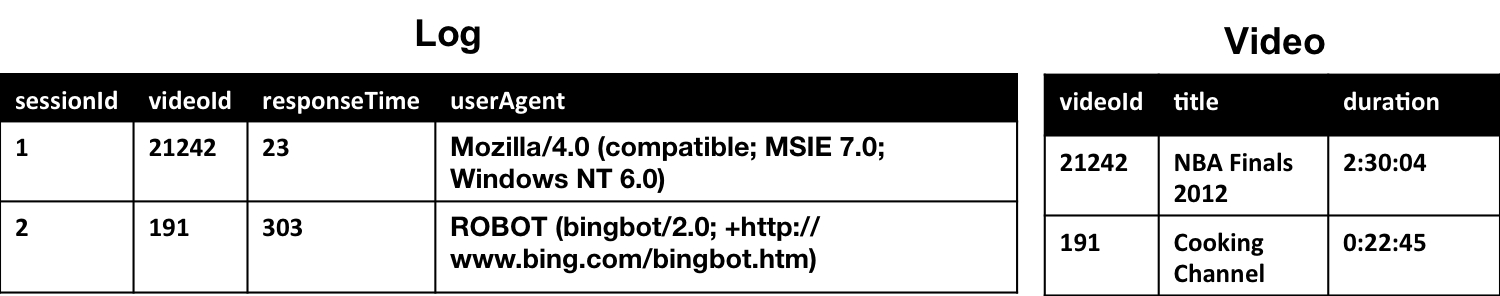
\includegraphics[width=\columnwidth]{figs/sample-clean-example.png}\vspace{-0.25em}
 \caption{A simplified log analysis example dataset. In this dataset, there are two tables: a fact table representing video views and a dimension table representing the videos.\label{example-1}}\vspace{-1em}
\end{figure}

\subsection{Running Example: Log Analysis}
To illustrate our framework, we use the following running example which is a 
simplified schema of one of our experimental datasets (Figure~\ref{example-1}).
Imagine, we are querying logs from a video streaming company. 
These logs record visits from users as they happen and grow over time.
We have two tables, \tbl{Log} and \tbl{Video}, with the following schema:

\begin{lstlisting}[mathescape]
Log(sessionId$\textrm{,}$ videoId$\textrm{,}$ responseTime$\textrm{,}$ userAgent)
Video(videoId$\textrm{,}$ title$\textrm{,}$ duration)
\end{lstlisting}
These tables are related with a foreign-key relationship between
Log and Video.
Though SVC supports inserts, deletions, and updates, for clarity in our example, we consider insertions
into Log which is cached in a temporary table:

%\reminder{I replace LogInserts with LogIns for saving a line of space. Make sure it is consistent in the whole paper.}
\begin{lstlisting}[mathescape]
LogIns(sessionId$\textrm{,}$ videoId$\textrm{,}$ responseTime$\textrm{,}$ userAgent)
\end{lstlisting}


\subsection{Materialized View Maintenance}\label{subsec-inc}
Views define logical relations which can be queried instead of physical base relations.
MVs are a class of views that are pre-computed and stored (i.e materialized).
Any form of pre-computed, derived data encounters the problem of staleness when the physical base relations update.

One approach to this problem is to recompute the materialized view every time there are updates to the base tables.
However, this approach is very inefficient if updates to the data generally have small or sparse effect on the MV. 
A contrasting approach is incremental view maintenance (IVM), where rows in the MV are incrementally updated based on the updates to the base table.
Incremental maintenance of MVs has been well studied; see \cite{chirkova2011materialized} for a survey of the approaches. 
At a high-level, incremental maintenance algorithms typically consist of the following steps: (1) maintain a cache of insertions and deletions for each physical base table, then using the view definition derive a \emph{change propagation formula} in terms of the set of insertions and deletions, and finally apply the formula to the view.
For a variety of view types, these rules are described in detail in \cite{DBLP:journals/vldb/KochAKNNLS14, DBLP:conf/pods/Koch10}.

Incremental maintenance may not be efficient in all cases.
Consider the view that calculates the median \tbl{responseTime} grouped by \tbl{userAgent} on our running example dataset.
In general, to ensure correctness, the view has to store the entire set of \tbl{responseTime} attributes for each group to allow for incremental maintenance.
Along the lines of this example, there are cases when recomputation may require less storage of state or even less computation.
Thus, materialized views are maintained either with incremental maintenance, recomputation, or a mix.




 


\iffalse
Incremental maintenance may not be efficient in all cases.
Consider the view that calculates the median \tbl{responseTime} grouped by \tbl{userAgent} on our running example dataset.
In general, to ensure correctness, the view has to store the entire set of \tbl{responseTime} attributes for each group to allow for incremental maintenance.
Along the lines of this example, there are cases when recomputation may require less storage of state or even less computation.
Thus, materialized views are maintained either with incremental maintenance, recomputation, or a mix.



\subsubsection{Practical Considerations}
The algebraic analysis of incremental maintenance \cite{DBLP:journals/vldb/KochAKNNLS14, DBLP:conf/pods/Koch10} informs us which views can be incrementally maintained efficiently.
However, there are many practical considerations of executing these operations in real database systems and it may not always be feasible to immediately apply updates; even if theoretically possible.
The main problem is that while immediate incremental maintenance has many advantages, the particulars of the database system and available resources often dictate how updates are propagated. 

\fi

\subsubsection{Practical Considerations}

In real-world systems, for large datasets or fast data update rate, it may not always be feasible to maintain MVs immediately. Therefore, deferred maintenance is an alternative and often preferred solution.
The main insight of deferral is to avoid maintaining the view immediately and to schedule an update at a more convenient time either in a pre-set way or adaptively.
In deferred maintenance approaches, the user often accepts some degree of staleness for additional flexibility in scheduling.
These costs can also be deferred to query execution time.
In particular, we highlight a technique called lazy maintenance which applies updates to the view only when a user's query requires a row \cite{zhou2007lazy}.
While always fresh, both lazy maintenance and immediate maintenance hit a bottleneck when there are rapid updates, and this results increasingly degraded performance if a user wants to query a view.
The alternative is a periodic strategy, but this means that there is unbounded error on queries between maintenance periods.

The data cleaning perspective that SVC offers on this problem is that there is a tradeoff between accuracy and computation.
By using sampling, we give the user access to a new tradeoff space between immediate (or close to immediate, i.e., mini-batch) maintenance and long-periodic maintenance.

\subsection{SampleClean: Fast and Accurate Query Processing on Dirty Data}
In our prior work on the SampleClean project \cite{wang1999sample}, we proposed a framework for scalable data cleaning.
Similar to the accuracy-performance contrast between immediate maintenance and periodic maintenance in the materialized view setting, data cleaning also faces a similar challenge.
Traditionally, data cleaning has explored expensive, up-front cleaning of entire datasets for increased query accuracy, and those who were unwilling to pay the full cleaning cost avoided data cleaning altogether.
We proposed SampleClean to add an additional tradeoff to this design space by using sampling.

SampleClean (Figure \ref{sc}) has three parts: (1) sampling, (2) data cleaning, and (3) query result estimation.
First, SampleClean creates a sample of dirty data (which are erroneous, missing, or otherwise corrupted records).
Then, the framework applies a data cleaning procedure to the sample.
Finally, when users query the dataset, the framework uses the clean sample to extrapolate clean query results.
In this work, the main challenge was that data cleaning can potentially change the statistics of a sample and the queries need to compensate for those effects.
In our initial work, SampleClean mainly focused on three common aggregates: \sumfunc, \avgfunc, and \countfunc queries.

The SampleClean project showed that there were two contrasting approaches to query processing on a sample of cleaned data.
We could (1) clean the sample first and then run the query on the sample, or (2) look at the difference between the clean and dirty samples and calcuate a correction to correct an existing dirty result. 
Approach (1) is similar to those studied in the Approximate Query Processing (AQP) literature \cite{OlkenR86,AgarwalMPMMS13, joshi2008materialized}; however in cases when data errors were small, we found that the approximation error dominated.
To address this problem, we developed approach (2), which we called \nsc, and we found that \nsc was more accurate in mostly clean datasets as it leverages existing deterministic results leading to reduced approximation error.
In the materialized view setting, we found that \nsc led to more accurate results in our experiments (see Section \ref{exp}). 

\begin{figure}[t] \vspace{-2em}
\centering
 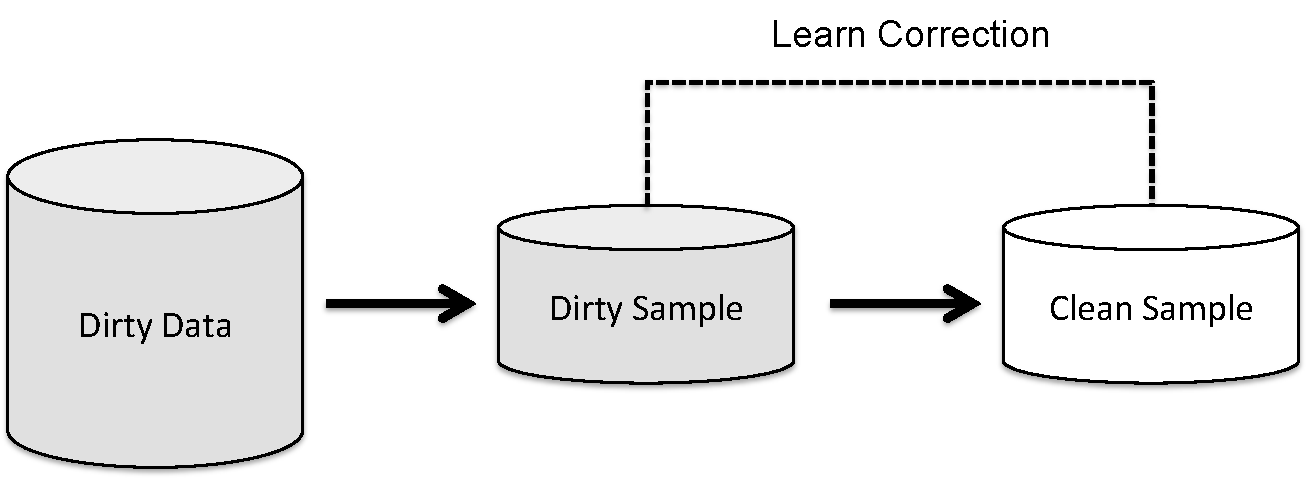
\includegraphics[scale=0.30]{figs/sys-arch2.pdf} \vspace{-.25em}
 \caption{A basic overview of SampleClean. SampleClean uses a random sample of dirty data to learn how a data cleaning algorithm affects queries on the sample. We can then derive a correction to compensate for the dirtiness.\label{sc}}\vspace{-1.75em}
\end{figure}

\subsection{New Challenges}
Inspired by SampleClean, SVC samples a stale view, cleans the sample view by restricting the maintenance to just the rows in the sample, and then applies \nsc to correct the results of queries on the stale view.
Applying this data cleaning framework to the materialized view setting leads to some interesting theoretical challenges with new insights for both materialized view maintenance and data cleaning.
In SampleClean, we simply treated the data cleaning as a black box and did not study how to clean a dirty sample data. However, in SVC, we cannot make such assumption and have to devise efficient data-cleaning techniques to ``clean" a stale sample view. 

Staleness is a new type of data error.
In materialized views, staleness can lead to rows that are missing from the ``dirty" view or conversely need to be deleted. These issues pose new challenges in  query correction. 
We further explore and formalize the class of queries that SVC can support.
We extend the generality of the framework to support queries than the \sumfunc, \avgfunc, and \countfunc which studied before.

Sampling is particularly sensitive to variance in the dataset, and large outliers can significantly reduce query accuracy.
In this work, we give an explicit treatment of outliers records. 




